%%%%%%%%%%%%%%%%%%%%%%%%%%%%%%%%%%%%%%%%%%%%%%%%%%%%%%%%%%%%%%%%%%%%%%%%%%%%%%%%
%2345678901234567890123456789012345678901234567890123456789012345678901234567890
%        1         2         3         4         5         6         7         8

%\documentclass[letterpaper, 10 pt, conference]{ieeeconf}  % Comment this line out if you need a4paper

\documentclass[a4paper, 10pt, conference]{ieeeconf}      % Use this line for a4 paper

\IEEEoverridecommandlockouts                              % This command is only needed if 
                                                          % you want to use the \thanks command

\overrideIEEEmargins                                      % Needed to meet printer requirements.

% See the \addtolength command later in the file to balance the column lengths
% on the last page of the document

% The following packages can be found on http:\\www.ctan.org
\usepackage{graphicx} % for pdf, bitmapped graphics files
\usepackage{caption} % for captions
%\usepackage{epsfig} % for postscript graphics files
%\usepackage{mathptmx} % assumes new font selection scheme installed
%\usepackage{times} % assumes new font selection scheme installed
%\usepackage{amsmath} % assumes amsmath package installed
%\usepackage{amssymb}  % assumes amsmath package installed

\title{\LARGE \bf
Exercise 2 - Localisation\\
Intelligent Robotics \\
PENNY
}


\author{Federico Bacci, Daniel Clark, Laura Ferrante, Alessandro Pozzer, Saif Sidhik and Milan Mariya Tomy
}


\begin{document}



\maketitle
\thispagestyle{empty}
\pagestyle{empty}


%%%%%%%%%%%%%%%%%%%%%%%%%%%%%%%%%%%%%%%%%%%%%%%%%%%%%%%%%%%%%%%%%%%%%%%%%%%%%%%%
\begin{abstract}

This report introduces different probabilistic algorithms for mobile robot localisation given a map of the environment. Among the algorithms tested are the Monte Carlo localisation algorithm and its variant, Adaptive Monte Carlo Localisation. After tuning the algorithms’ parameters, experimental data was gathered for each algorithm to compare their suitability for the task. The results were then analysed to verify the performance of each algorithms and compare them with the AMCL implementation provided by ROS Nav Stack.
\end{abstract}

%%%%%%%%%%%%%%%%%%%%%%%%%%%%%%%%%%%%%%%%%%%%%%%%%%%%%%%%%%%%%%%%%%%%%%%%%%%%%%%%
\section{Aims}
The aim of this project was to implement a ROS node for Monte-Carlo Localisation (MCL) and Adaptive Monte-Carlo Localisation (AMCL) which uses a particle filter to localize the robot in a given map, optimally combine unreliable evidence to estimate the position of a robot - which has unreliable sensing and motion- using a discretized state of belief (particles). 

\section{Algorithms}
For this project we extended an abstract class which provided most of the functionality for the particle filter. We were left to implement three functions, one which generated the initial particle cloud, one which updated the particle cloud after each time step and one which generated an estimated position for the robot from the particle cloud data.
\subsection{Initialise Particle Cloud}
This function simply distributes the chosen number of particles over a wide area, in a Gaussian distribution around an initial pose given by the user. This wide spread helps to localise the robot even if the initial pose is incorrect.
\subsection{Update Particle Cloud}
This function used Roulette Wheel Sampling, based on likelihoods taken from the given sensor model, to generate a new particle cloud. The new particle cloud will mostly be made up of particles from the previous timestep. The majority of these particles are ones which were given a high likelihood, however particles with lower likelihoods were also chosen to help add noise to the system and correct for errors in the model. This way by filtering particles with low likelihoods, the robot can be more confident in its location.

Gaussian and Von Mises noise was then added to each particle. This ensures that the robot can remain localised despite a map which is not perfect, an incorrect motion model, and noisy sensor data.

In the case of AMCL, the number of particles is adjusted based on the sum of the likelihoods and a confidence threshold. Particles are chosen, again using Roulette Wheel Sampling and the value is summed until the total is greater than the confidence threshold. If all the particles are summed and the threshold is still not reached, new particles are generated in the same way new particles are generated in each time step until the threshold is reached.

%In addition to the standard AMCL algorithm, extra steps were added such that as the number of particles increases, so does the amount of Gaussian noise added to each particles. This way is the filter has a low level of confidence, it will create a large number of particles with a large spread, as to more quickly find a pose in which it is confident.

\subsection{Estimate Pose}
Two techniques were implemented to calculate an estimated pose given the particle cloud.

\subsubsection{Global Averaging}
The first is to use a naive averaging function which simply takes the mean of all the positions and orientations in the particle cloud. 

\subsubsection{Clustering}
Two clustering algorithms were considered for use in this estimation technique. The first was K-Means clustering, and the second was Hierarchical Agglomerative Clustering (HAC). It was soon realised that K-Means is less suitable because the number of clusters in the particle cloud varies significantly depending on the similarity between various possible poses. HAC deals with this by changing the number of clusters, dependent on the distance between clusters in a generated hierarchy of clusters.
HAC is a method of cluster analysis in which each observation (in this case, each particle) starts in its own cluster, and pairs of clusters are merged until only one cluster remains.

In this project, the particles are clustered such that the variance within the cluster is minimised. This ensures that particles which are at similar poses are grouped into the same cluster. The agglomeration algorithm is cut off when the distances between clusters are above a certain limit. The limit ensures that clusters which are too far apart will not merge together. 

The algorithm chooses the ‘best’ cluster from the remaining clusters based on the highest cumulative weights of the particles in the clusters. The final pose is estimated to be the average of the poses of the particles in the ‘best’ cluster.

\section{Characterisation}
Initially, the parameters were deducted from simple observation. The parameters' tuning was achieved through properly designed experiments.

\subsection{Tuning Gaussian Standard Deviation}
Initially, the particles are given a wide distribution so that it can deal with a lack of a correct initial pose. At the required value, the noise is enough to cover the majority of the map. This enables correct localisation even with no initial pose.

For the update step, the Gaussian noise had to be such that the particles formed a dense cloud, but with enough noise such that it can recover from possible errors. Extremely high values for standard deviation such as 20, resulted in particles being outside the map. Low values such as 1 resulted in a very low spread of particles, which limited the robots ability to localise itself correctly. It was found that for large values, localisation did not take place, and so an appropriate low value was selected.

\subsection{Tuning Von Mises Noise}
The robot was put in a location of the map with a simple unambiguous pattern, then the robot was given an initial pose in the opposite direction. The time in which the Pioneer rotates around the yaw axis was recorded while increasing the value of Von Mises noise from 0.05 to 0.5. It was noticed that the robot never matched the actual orientation if the noise is too low, while for high values (from 0.3) the estimated pose kept oscillating wildly. By varying the values, the suitable value was found to be 0.1.

\begin{figure}[b]
\centering
\captionsetup{justification=centering}
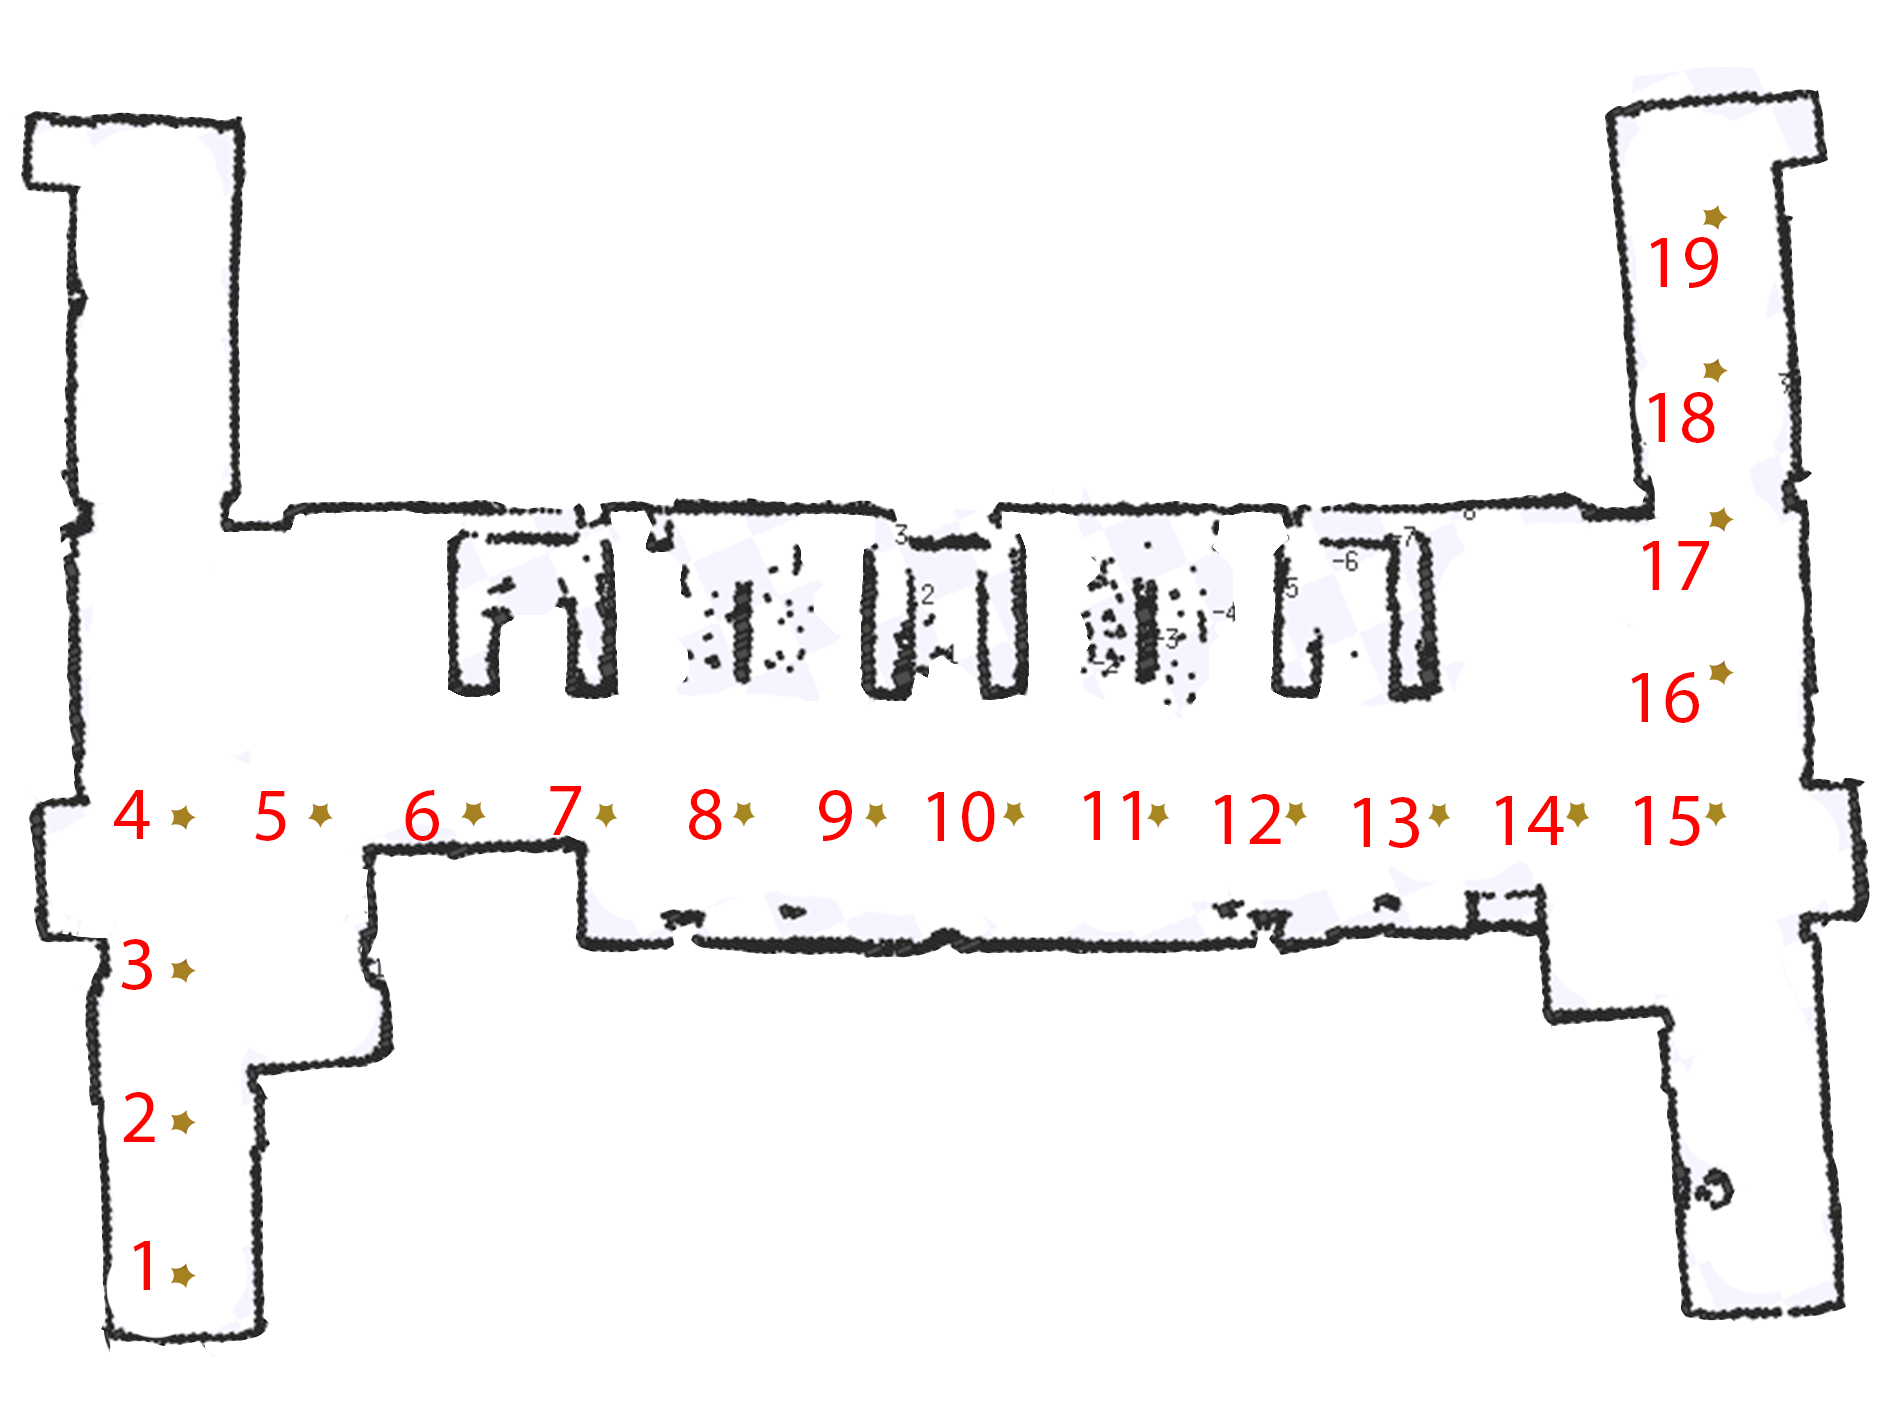
\includegraphics[scale=0.35]{ex2path}
\caption{Path used for Experiments}
\label{fig:map}
\end{figure}


\section{Hypotheses}
\begin{enumerate}

\item The first hypothesis is that the MCL-HAC more precisely localises the robot than the Mean Particle Filter. As the particle cloud results in a multi-modal distribution, a clustering algorithm would better approximate the estimated pose rather than a global mean which does not take into account the clusters formed. Hence, MCL-HAC would tend to give lower error values than the Global Mean Particle Filter.

\item The second hypothesis is that the AMCL-HAC is better than MCL-HAC at precisely localising the robot. AMCL should give lower error values because the smaller cloud size when it is more confident will reduce the amount of noise introduced into the estimate pose function.

\item The third hypothesis is that the AMCL-ROS can localise the robot more accurately than AMCL-HAC. This would be because AMCL-ROS has been tuned over long periods of time on various data sets, whilst AMCL-HAC has not.
 
\end{enumerate}
\section{Method}

The performance of MCL-GlobalMean, MCL-HAC, AMCL-HAC and the AMCL implementation in the ROS navstack (AMCL-ROS) were analysed by estimating the average error between the actual position of the robot and the predicted position of the robot. 
The experiments will be conducted in the lower ground floor, with points marked every 2 meters along a route, as shown in Fig.\ref{fig:map}. Firstly, the robot will be started from a specific point (Point 1 in Fig.\ref{fig:map}) which would give a high likelihood value. Then the robot will be made to track the route laid out in Fig.\ref{fig:map}. The initial position set in rviz will be the same as the actual location. The error in the estimated location of the robot in rviz, from its actual location will be read from a scaled map and recorded for data processing. This process was repeated 3 times for each algorithm.

\section{Results and Analyses}

From Fig.\ref{fig:linegraph}, it is evident that MCL-HAC algorithm has lower error values in areas of uncertainty (e.g. point 10) due to the fact that multiple clusters are generated and because of this, the mean value between the two clusters is a long way from the robot's actual location. With a confidence value of 95\%, 0.0044 was found to be the p-value for Hyp.1.

With a confidence value of 95\%, the p-value for Hyp.2 was found to be 0.0127. This means that the difference in errors between AMCL-HAC and MCL-HAC implementations is not statistically significant.

A confidence level of 95\% Hyp.3 had a p-value of 0.001 which is extremely significant. It shows that we can reject the null hypothesis, and confirm Hyp.3. From Fig.\ref{fig:linegraph} it is very evident that AMCL-ROS correctly localises the robot better than AMCL-HAC in almost all cases.

\begin{figure}[b]
\centering
\captionsetup{justification=centering}
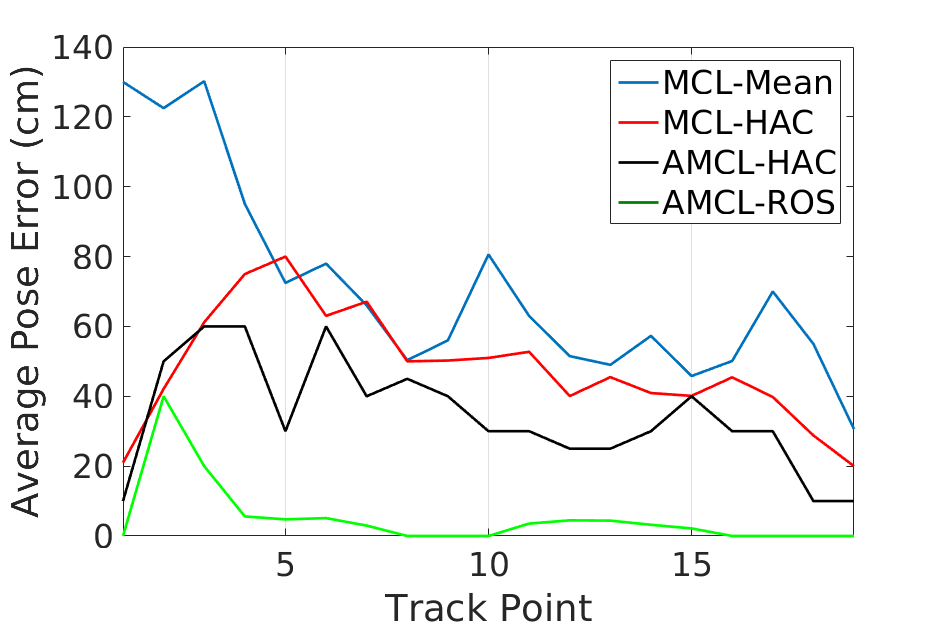
\includegraphics[scale=0.26]{PARTICLEFILT}
\caption{Average Errors For Different Algorithms}
\label{fig:linegraph}
\end{figure}

\section{Conclusions}
In conclusion, a clustering algorithm is a better choice for pose estimation than one which cannot deal with multi-modal distributions. The results also show that whilst AMCL is better at localisation than MCL, it requires significant tuning of parameters to to give a significant accuracy difference.
\end{document}